\documentclass[11pt,spanish,letterpaper]{article}
\usepackage[utf8]{inputenc}
\usepackage{babel}
\usepackage{fullpage}
\usepackage{listings}
\usepackage[sc]{mathpazo}
\usepackage{courier}
\usepackage{enumitem}
\usepackage{textcomp}
\usepackage{fancyhdr}
\usepackage{tikz}
\usepackage{microtype}
\usepackage{xfrac}
\usepackage{multicol}
\usepackage{tabularx}
\usepackage{vwcol} 
\usepackage{tikz}


\newcommand{\onelinerule}{\rule[2.3ex]{0pt}{0pt}}
\newcommand{\twolinerule}{\rule[6.2ex]{0pt}{0pt}}
\newcommand{\respuesta}{\framebox[\textwidth]{\twolinerule}}

%Nombre
\newcommand{\nombre}{
 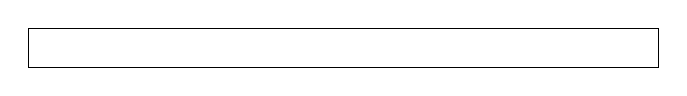
\begin{tikzpicture}[xscale=.4,yscale=.5]
   \draw (0, 0) rectangle (20, 1);
 \end{tikzpicture}%
}

%Rol
\newcommand{\rol}{
 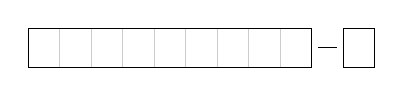
\begin{tikzpicture}[xscale=.4,yscale=.5]
   \draw[gray!40] ( 0, 0) grid      ( 9, 1);
   \draw          ( 0, 0) rectangle ( 9, 1);
   \draw          (10, 0) rectangle (11, 1);
   \draw (9 + .2, .5) -- (10 - .2, .5);
 \end{tikzpicture}%
}

%Paralelo
\newcommand{\para}{
 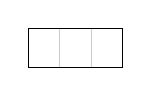
\begin{tikzpicture}[xscale=.4,yscale=.5]
   \draw[gray!40] ( 0, 0) grid      ( 3, 1);
   \draw          ( 0, 0) rectangle ( 3, 1);
 \end{tikzpicture}%
}

%Numero Pregunta
\newcommand{\li}{\lstinline}
\providecommand{\pond}[1]{[{\small\textbf{#1\%}}]}

\lstdefinelanguage{py}{%
 classoffset=0,%
   morekeywords={%
     False,class,finally,is,return,None,continue,for,lambda,try,%
     True,def,from,nonlocal,while,and,del,global,not,with,print,%
     as,elif,if,or,yield,assert,else,import,pass,break,except,in,raise},%
   keywordstyle=\color{black!80}\bfseries,%
 classoffset=1,
   morekeywords={int,float,str,abs,len,raw_input,exit,range,min,max,%
     set,dict,tuple,list,bool,complex,round,sum,all,any,zip,map,filter,%
     sorted,reversed,dir,file,frozenset,open,%
     array,zeros,ones,arange,linspace,eye,diag,dot},
   keywordstyle=\color{black!50}\bfseries,%
 classoffset=0,%
 sensitive=true,%
 morecomment=[l]\#,%
 morestring=[b]',%
 morestring=[b]",%
 stringstyle=\textit,%
}

\lstdefinelanguage{testcase}{%
 moredelim=[is][\bfseries]{`}{`},%
 %backgroundcolor=\color{gray!20},%
}

\lstdefinelanguage{file}{%
 frame=single,%
}

\lstset{language=py}
\lstset{basicstyle=\ttfamily}
\lstset{columns=fixed}
\lstset{upquote=true}
\lstset{showstringspaces=false}
\lstset{rangeprefix=\#\ }
\lstset{includerangemarker=false}
\lstset{
    escapeinside={(*}{*)}
}
\newlist{certamen}{enumerate}{1}
\setlist[certamen]{%
 label=\arabic*.,
 font=\LARGE\bfseries,%
 labelindent=-.5in,%
 leftmargin=0pt,%
 labelsep=1em%
}



\usetikzlibrary{shapes.geometric, arrows}

\tikzstyle{startstop} = [circle, minimum width=1cm, minimum height=1cm, text centered, draw=black, fill=yellow!30]
\tikzstyle{io} = [trapezium, trapezium left angle=70, trapezium right angle=110, minimum width=.3cm, minimum height=.3cm, draw=black, fill=green!30]
\tikzstyle{process} = [rectangle, minimum width=.3cm, minimum height=.3cm, draw=black, fill=blue!30]
\tikzstyle{decision} = [diamond, minimum width=.3cm, minimum height=.3cm, text centered, draw=black, fill=red!30]
\tikzstyle{arrow} = [thick,->,>=stealth]

\newcommand{\titulo}{Laboratorio 3 -- Semestre 2, 2018}

\pagestyle{fancy}
\lhead{
{\Large\bfseries Programación -- \titulo} %\hspace{1cm} Paralelo \para \\
%{\small
%\begin{tabular}{ll}
%Nombre & \nombre \hspace{.3cm} Rol \rol \\
%Nombre & \nombre \hspace{.3cm} Rol \rol \\
%Nombre & \nombre \hspace{.3cm} Rol \rol \\
%\end{tabular}}
}
\chead{}\rhead{}\lfoot{}\cfoot{}\rfoot{}
\renewcommand{\headrulewidth}{0pt}
\addtolength{\headheight}{12ex}
%\headsep=5ex

\setlength\parindent{0pt}

%\input{encabezado.tex}
%\input{definiciones.tex}

\begin{document}

Se tienen archivos .txt con libros. Por ejemplo el quijote y moby-dick se encuentran en los archivos quijote.txt y moby-dick.txt respectivamente:
\\
\begin{minipage}[T]{21em}
  \centering
quijote.txt
  \begin{lstlisting}[basicstyle=\ttfamily\small, frame = single]
En un lugar de la Mancha, de cuyo
nombre no quiero acordarme, no ha
mucho tiempo que vivia un hidalgo
de los de lanza en astillero, 
adarga antigua, rocin flaco y 
galgo corredor. Una olla de algo 
mas vaca que carnero
...
  \end{lstlisting}
\end{minipage}
\hfill
\begin{minipage}[T]{20em}
  \centering
moby-dick.txt
  \begin{lstlisting}[basicstyle=\ttfamily\small, frame = single]
Call me Ishmael. Some years ago never
mind how long precisely having little
or no money in my purse, and nothing 
particular to interest me on shore, I
thought I would sail about a little 
and see the watery part of the world.
...
  \end{lstlisting}
\end{minipage}

Desarrolle una aplicación que me permita ingresar los nombres de los archivos .txt de estos libros infinitamente y me muestre las $n$ palabras más frecuentes (que aparecen más veces en el libro), siendo $n$ un número entero positivo ingresado por el usuario. La aplicación termina cuando se ingresa fin como nombre de archivo de libro. Guíese por los ejemplos:

 \begin{lstlisting}[language=testcase, frame=single]
Ingrese tiempo: (*\textbf{00:00:05}*)
Ingrese nombre del archivo del libro:(*\textbf{quijote.txt}*)
de
que
los
y
la
Ingrese nombre del archivo del libro:(*\textbf{moby-dick.txt}*)
Ingrese n:(*\textbf{3}*)
the
i
and
Ingrese nombre del archivo del libro:(*\textbf{fin}*)
 \end{lstlisting}

En el siguiente ejemplo se colocan puntos suspensivos para señalar que existen más líneas entremedio:
 
 \begin{lstlisting}[language=testcase, frame=single]
Ingrese nombre del archivo del libro:(*\textbf{moby-dick.txt}*)
Ingrese n:(*\textbf{2}*)
the
i
Ingrese nombre del archivo del libro:(*\textbf{moby-dick.txt}*)
Ingrese n:(*\textbf{5}*)
the
i
and
to
me
Ingrese nombre del archivo del libro:(*\textbf{fin}*)
 \end{lstlisting}
\end{document}

